\input{../include/preamble}

\title[ID1019 Higher order]{Higher order}


\author{Johan Montelius}
\institute{KTH}
\date{\semester}

\begin{document}

\begin{frame}
\titlepage
\end{frame}

\begin{frame}{let's play some cards}

\begin{columns}

 \begin{column}{0.2\linewidth}
   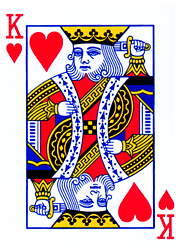
\includegraphics[width=\linewidth]{kung.png}
 \end{column}
 
 \pause

 \begin{column}{0.8\linewidth}
  \begin{itemize}
   \item ${\rm Suit} \in \{{\rm spade}, {\rm heart}, {\rm diamond}, {\rm club}\}$
   \pause
   \item ${\rm Value} \in \{2,3,\ldots 14\}$
   \pause 
   \item ${\rm card}$ = \{card, Suit, Value\}
  \end{itemize}
 \end{column}
\end{columns}

\end{frame}

\begin{frame}[fragile]{order of cards}

\pause
\begin{verbatim}
lt({card, S, V1}, {card, S, V2})  ->   V1 < V2;
\end{verbatim}
\pause
\begin{verbatim}
lt({card, club, _}, _) ->   true.
\end{verbatim}
\pause
\begin{verbatim}
lt({card, diamond, _}, {card, heart, _}) ->   true;
\end{verbatim}
\pause
\begin{verbatim}
lt({card, diamond, _}, {card, spade, _}) ->   true;
\end{verbatim}
\pause
\begin{verbatim}
lt({card, heart, _}, {card, spade, _}) ->   true; 
\end{verbatim}
\pause
\begin{verbatim}
lt({card, _, _}, {card, _, _}) ->   false.
\end{verbatim}

\end{frame}

\begin{frame}[fragile]{sorting cards}

\begin{columns}

 \begin{column}{0.5\linewidth}
\begin{verbatim}
sort([]) -> 
   [];
\end{verbatim}
\pause
\begin{verbatim}
sort(Cards) -> 
   {C1, C2} = split(Cards),
   S1 = sort(C1),
   S2 = sort(C2),
   merge(S1, S2).
\end{verbatim}
 \end{column}
 
 \pause

 \begin{column}{0.5\linewidth}
\begin{verbatim}
split([]) ->
   {[], []};
\end{verbatim}
\pause
\begin{verbatim}
split([C|S]) ->
    {H1, H2} = split(S),
    {..., ...}.
\end{verbatim}
 \end{column}
\end{columns}

\end{frame}

\begin{frame}[fragile]{tail recursive split}

\begin{columns}

 \begin{column}{0.5\linewidth}
\begin{verbatim}
split([]) ->
   {[], []};
\end{verbatim}
\pause
\begin{verbatim}
split([C|S]) ->
    {H1, H2} = split(S),
    {..., ...}.
\end{verbatim}
 \end{column}
 
 \pause

 \begin{column}{0.5\linewidth}
\begin{verbatim}
split(Deck) ->
   split(Deck, [], []).
\end{verbatim}

\pause
\begin{verbatim}
split([], D1, D2) ->
   {D1, D2};
\end{verbatim}
\pause
\begin{verbatim}
split([C|S], D1, D2) ->
   split(S, ..., ...).
\end{verbatim}
 \end{column}
\end{columns}

\end{frame}

\begin{frame}[fragile]{sorting cards}

\begin{verbatim}
merge([], S2) ->  ...;
merge(S1, []) ->  ...;
\end{verbatim}
\pause
\begin{verbatim}
merge([C1|S1], [C2|S2]) -> 
   case lt(C1, C2) of
     true -> 
        [C1 | merge(S1, [C2|S2])];
     false
        [C2 | merge([C1|S1], S2)]
   end.
\end{verbatim}

\end{frame}

\begin{frame}{what to do}

\pause Implement function that sorts names of people.

\pause Implement function that sorts a frequency table.

\pause Implement function that sorts ....


\end{frame}

\begin{frame}[fragile]{old friends}

Have we seen this before?

\pause\vspace{20pt}
\begin{columns}
   \begin{column}{.5\linewidth}
     \begin{block}{sum/1}
       \begin{verbatim}
sum([]) ->
   0;
sum([H|T]) ->
    add(H,sum(T)).
       \end{verbatim}
       \vfill
     \end{block}
   \end{column} 
\pause
   \begin{column}{.5\linewidth}
     \begin{block}{prod/1}
       \begin{verbatim}
prod([]) ->
   1;
prod([H|T]) ->
   mul(H,prod(T)).
       \end{verbatim}
       \vfill
     \end{block}
   \end{column}
  \end{columns}

\vspace{20pt}{\em There is no built-in add/2, nor mul/2, but we can pretend that there is.}

\end{frame}



\begin{frame}[fragile]{good to have}

We would like to to this:

\pause\vspace{20pt}

\begin{columns}
   \begin{column}{.5\linewidth}
     \begin{block}{foldr/3}
       \begin{verbatim}
foldr(Op, Acc, []) ->
   Acc;
       \end{verbatim}
\pause
       \begin{verbatim}
foldr(Op, Acc, [H|T]) ->
   Op(H, foldr(Op, Acc, T)).
      \end{verbatim}
       \vfill
     \end{block}
   \end{column}
\pause
   \begin{column}{.5\linewidth}
     \begin{block}{sum/1}
       \begin{verbatim}
sum(L) -> 
   Add = ...,
   foldr(Add, 0, L).
       \end{verbatim}
     \end{block}
\pause     
   \begin{block}{prod/1}
       \begin{verbatim}
prod(L) -> 
   Mul = ...,
   foldr(Mul, 1, L).
       \end{verbatim}
     \end{block}
   \end{column}
  \end{columns}

\pause\vspace{20pt}
{\em only problem, \ldots How do we express the function?}

\end{frame}

\begin{frame}[fragile]{lambda expressions}

We introduce a new data structure: a closure

  \vspace{20pt}

  \begin{tabular}{r l l}
   {\em Atoms} & = & \{a, b, c, \ldots\} \\
   {\em Closures} & = & \{f:e | f $\in $ Functions $\wedge$  e $\in $ Environment \}\\
   {\em Structures} & = & {\em Closures} $\cup$ {\em Atoms} $\cup$ \{ \{a, b\} \textbar a $\in$ {\em Structures}  $\wedge$  b $\in$ {\em Structures} \}
  \end{tabular}

\pause\vspace{10pt}
A {\em closure} is a function and an environment.

\pause\vspace{10pt}
We have not really defined what a {\em function} is nor an {\em environment} but let's forget this for a while.

\end{frame}

\begin{frame}[fragile]{function expressions}

\begin{code}
   <function> &::= 'fun' '(' <parameters> ')' '->' <sequence> 'end'\\
   <parameters> &::= '  ' | <variables> \\
   <variables> &::= <variable> |  <variable> ',' <variables>\\
\end{code}
\pause
\begin{code}
   <application> &::= <expression> '(' <arguments> ')'\\
   <arguments> &::= '  ' | <expressions> \\
   <expressions> &::= <expression> |  <expression> ',' <expressions>\\
\end{code}
\pause
\begin{code}
   <expression> &::= <function> | <application> | ...\\
\end{code}

\end{frame}

\begin{frame}[fragile]{function expressions}

\pause\vspace{10pt}
We will write:
\pause\vspace{40pt}\hspace{60pt}\verb!X = 2, F = fun(Y) -> {X,Y} end, F(4) !

\end{frame}


\begin{frame}[fragile]{evaluation of a function}

  \begin{itemize}
   \pause\item $E\sigma({\rm f})  \rightarrow  {\rm function}:\theta$ if
    \begin{itemize} 
           \pause\item $\mathrm{function}$ is the corresponding function of $f$
           \pause\item $\theta = \{ v/s \mid  v/s \in \sigma \wedge v {\rm\ free\  in\ f}\}$
    \end{itemize} 
  \end{itemize} 

\pause\vspace{20pt}

\begin{verbatim}
  X = 2, Y = 3, Z = 4, C = fun(V) -> V + Y end, ...
\end{verbatim}

{\em What is C?}


\end{frame}

\begin{frame}[fragile]{evaluation of an application}

  \begin{itemize}
   \pause\item $E\sigma(e(e_1, \ldots)) \rightarrow E\{v_1/s_1, \ldots\}\cup\theta({\rm sequence} )$ if
    \begin{itemize}        
           \pause\item $E\sigma(e) \rightarrow f:\theta$
           \pause\item ${\rm f} = {\rm fun}(v_1, \ldots) \rightarrow  {\rm sequence}$ 
           \pause\item $E\sigma(e_i) \rightarrow s_i$ 
    \end{itemize} 
  \end{itemize}

\pause\vspace{20pt}

\begin{verbatim}
   Y = 3, F = fun(V) -> V + Y end, F(4)
\end{verbatim}

\end{frame}
 
\begin{frame}[fragile]{example}

\begin{verbatim}
   foo(X) -> 
        Y = 3, 
        fun(V) -> V + Y + X end.
\end{verbatim}
\pause\vspace{20pt}

\begin{verbatim}
   F = foo(2), Y = 7, F(1)
\end{verbatim}
\end{frame}

\begin{frame}[fragile]{case closed}

\pause
     \begin{block}{sum/1}
       \begin{verbatim}
sum(L) -> 
  Add = fun(X,Y) -> X + Y end,
  foldr(Add, 0, L).
       \end{verbatim}
     \end{block}
   \pause
     \begin{block}{prod/1}
       \begin{verbatim}
prod(L) -> 
  Mul = fun(X,A) -> X * A end,
  foldr(Mul, 1, L).
       \end{verbatim}
\vfill
     \end{block}

\end{frame}

\begin{frame}[fragile]{example}

\pause What is gurka/1 doing?

\pause\vspace{20pt}

\begin{verbatim}
  gurka(L) -> 
    F = fun(_, A) -> A + 1 end,
    foldr(F, 0, L).
\end{verbatim}

\pause\vspace{20pt}
\pause How about tomat/1 doing?

\pause\vspace{10pt}
\begin{verbatim}
  tomat(L) -> 
    F = fun(H, A) ->  A ++ [H] end,
    foldr(F, [], L).
\end{verbatim}
\end{frame}

\begin{frame}[fragile]{example}
     \begin{block}{foldr/3}
       \begin{verbatim}
foldr(Op, Acc, []) ->
   Acc;
foldr(Op, Acc, [H|T]) ->
   Op(H, foldr(Op, Acc, T)).
       \end{verbatim}
       \vfill
     \end{block}
\pause

     \begin{block}{foldl/3}
       \begin{verbatim}
foldl(Op, Acc, []) ->
   Acc;
foldl(Op, Acc, [H|T]) ->
   foldl(Op, Op(H, Acc), T).
       \end{verbatim}
     \end{block}
\end{frame}


\begin{frame}[fragile]{example}

\pause\vspace{10pt}
\begin{verbatim}
  tomat(L) -> 
    F = fun(H, A) ->  A ++ [H] end,
    foldr(F, [], L).
\end{verbatim}
\pause 
\begin{verbatim}
  morot(L) -> 
    F = fun(H, A) ->  [H|A] end,
    foldl(F, [], L).
\end{verbatim}
\end{frame}

\begin{frame}{left or right}

Which one should you use, {\em fold-left} or {\em fold-right}?

\end{frame}

\begin{frame}[fragile]{append all}

\pause Append all lists in a lists.

\vspace{20pt}

\begin{verbatim}
appendl(L) ->
    F = fun(E,A) -> A ++ E end,
    foldl(F, [], L).
\end{verbatim}

\begin{verbatim}
appendr(L) ->
    F = fun(E,A) -> E ++ A end,
    foldr(F, [], L).
\end{verbatim}

\end{frame}



\begin{frame}{patterns}

In the {\tt lists} module. 

\begin{itemize}
\item {\tt map(F, List)}: return the list of F(X) for each element X in the list
\pause
\item {\tt filter(F, List)}: return a list of all elements X, for which F(X) evaluates to true
\pause
\item {\tt partition(F, List)}: partition the list based on the function F
\pause
\item {\tt zip(F, List1, List2)}: return a list of F(X1,X2)
\pause
\item {\tt sort(F, List)}: sort the list given that the function is less than or equal
\end{itemize}

\end{frame}


\begin{frame}[fragile]{an infinite list}

\pause\vspace{20pt}

\verb+Inf = infinity()+\pause \verb+, [0|Inf1] = Inf()+\pause \verb+, [1|Inf2] = Inf1()+

\pause
\begin{verbatim}
infinity() -> fun() -> infinity(0) end.
\end{verbatim}
\pause
\begin{verbatim}
infinity(N) -> [...|...].
\end{verbatim}

\end{frame}


\begin{frame}[fragile]{the list of fibonacci }

A function that returns an infitie list of Fibonacci numbers.

\pause\vspace{20pt}

\begin{verbatim}
fib() -> fun() -> fib(1,1) end.
\end{verbatim}
\pause
\begin{verbatim}
fib(F1, F2) -> [F1 | fun() -> fib(F2, F1+F2) end].
\end{verbatim}

\pause\vspace{20pt}

\begin{verbatim}
\end{verbatim}

\end{frame}

\begin{frame}{Higher order}

Order of what?

\pause\vspace{20pt}
A first order function takes a value, a data structures, as argument and returns a value.

\pause\vspace{20pt}
A second order function takes a first order function as argument or returns a first order function.

\pause\vspace{20pt}
A third order function ....

\pause\vspace{20pt}
Higher order functions takes a higher order ...

\pause\vspace{20pt}
Are functions considered to be ``first-class citizen''?
\end{frame}


\begin{frame}{not really}

\vspace{40pt}Not really - look at this.

\end{frame}

\begin{frame}{set comprehension}

In mathematics, {\em set comprehension}:

$$l = \lbrace 1,2,3,4,5,6,7,8 \rbrace ,  k = \lbrace 2*x | x \in l \wedge x < 5 \rbrace$$

\pause In functional programming, {\em list comprehension}:

\pause 
\vspace{20pt}\hspace{40pt} {\tt L = [1,2,3,4,5,6,7,8], K = [X*2 || X <- L, X < 5]}


\end{frame}

\begin{frame}[fragile]{quick sort}

\begin{verbatim}
qsort([]) -> [];
qsort([P|L]) ->
    Lower = [X||X <- L, X < P],
    Higher = [X||X <- L, X >= P],
    qsort(Lower) ++ [P | qsort(Higher)].
\end{verbatim}


\end{frame}


\begin{frame}{Summary}

\pause Higher order programming:


\begin{itemize}
\pause\item {closure}: a function and an environment
\pause\item {generic algorithms}: separate the recursive pattern from the data it operates over
\pause\item {continuations}: powerful technique to handle incomplete information
\pause\item {list comprehension}: very compact syntax for the construction of lists
\end{itemize}


\end{frame}


\end{document}



